\documentclass[dvipdfmx, 8pt, aspectratio=169]{beamer}
\usepackage{graphicx}
\usepackage{amsmath}
\usepackage{amssymb}
\usepackage{ascmac}
% \usepackage{txfonts}
\usepackage{url}
\usepackage{bm}
\usepackage{booktabs}
\usepackage[caption=false, font=footnotesize]{subfig}
\usepackage{xcolor}

\usepackage{tikz}
\usetikzlibrary{calc}
\usetikzlibrary{intersections}
\usetikzlibrary{shapes}

\definecolor{mri-blue}{RGB}{0, 59, 131}
\definecolor{mri-blue0}{RGB}{0, 25, 66}
\definecolor{mri-blue1}{RGB}{60, 130, 245}
\definecolor{mri-blue2}{RGB}{128, 174, 248}
\definecolor{mri-blue3}{RGB}{226, 236, 253}
\definecolor{mri-red0}{RGB}{66, 0, 17}
\definecolor{mri-red1}{RGB}{220, 0, 60}
\definecolor{mri-red2}{RGB}{236, 115, 148}
\definecolor{mri-red3}{RGB}{250, 217, 226}
\definecolor{mri-gray1}{RGB}{89, 87, 87}
\definecolor{mri-gray2}{RGB}{147, 146, 146}
\definecolor{mri-gray3}{RGB}{230, 230, 230}
\definecolor{mri-green1}{RGB}{0, 66, 41}
\definecolor{mri-green1}{RGB}{50, 155, 115}
\definecolor{mri-green2}{RGB}{122, 190, 164}
\definecolor{mri-green3}{RGB}{224, 240, 234}
\definecolor{mri-yellow0}{RGB}{66, 49, 0}
\definecolor{mri-yellow1}{RGB}{220, 160, 0}
\definecolor{mri-yellow2}{RGB}{232, 193, 89}
\definecolor{mri-yellow3}{RGB}{248, 236, 204}

\usetheme{Copenhagen}
\usefonttheme{professionalfonts}
\setbeamertemplate{navigation symbols}{}
\setbeamercolor{structure}{fg=mri-blue}
\setbeamercolor{alerted text}{fg=mri-red1}
\setbeamercolor{example text}{fg=mri-green1}


\title{第一級陸上無線技術士 攻略資料}
\author{近藤 綜太}
\date{}

\begin{document}

\frame{\maketitle}

\begin{frame}[t]
  \frametitle{基礎}
  \framesubtitle{一様分布する電荷による電界}

  \textcolor{mri-blue}{
  \textbf{電荷、電気力線、電界のイメージを理解することで解答できる。
  電気力線は電荷から湧き出す流線というイメージから、ガウスの法則の意味する内容が理解できる。
  \vspace{1zh}
  }
  }

  \begin{columns}[]
    \begin{column}{0.55\textwidth}
      ガウスの法則は、ある閉曲面を垂直に貫く電気力線の本数は、
      閉曲面の内部の電荷$Q$比例し、誘電率を$\varepsilon$とすると$Q/\varepsilon$と等しいという法則である。

      球体状に一様に分布する正電荷の中心と同じ中心を持つ球面を考えると、球面上の任意の点Pで電界は等しくなる\footnote{対称なので。}。
      点Pでの電界を$E$とし、電界が電気力線の面積密度であることを用いると、ガウスの法則より以下の式を得る。
      \begin{equation}
        4\pi r^{2} E = Q/\varepsilon
      \end{equation}
      正電荷の分布する範囲より小さな閉曲面を考えても同様で、閉曲面内部の電荷を$Q$とすればよい。
      \begin{equation}
        4\pi r^{2} E = \frac{1}{\varepsilon}  \cdot \frac{r^{3}}{r_{a}^{3}} \cdot Q
      \end{equation}

    \end{column}
    \begin{column}{0.4\textwidth}
      \centering
      \begin{figure}[t]
        \centering
        \begin{tikzpicture}[scale = 0.5]\footnotesize
          \coordinate (origin) at (0, 0);
          \coordinate (p) at (30:1.5);
          \draw[fill, ball color=mri-gray3, draw] (origin) circle[radius=2cm];
          \fill[ball color=mri-red1, opacity=.3] (origin) circle[radius=0.9cm];

          \draw[fill] (origin) circle[radius=1.5pt] node[below]{原点};
          \draw[fill] (p) circle[radius=1.5pt] node[below=1pt]{点P};
          \draw[thick, ->] ($(origin)!0.7!(p)$) -- ($(origin)!1.5!(p)$) node[above right]{$E$};
          \draw[thick, latex-latex] (origin) -- node[above=3pt]{半径$r$} (150:2) ;

          \draw[thin] (-30:1.8) -- (-30:2.8) node[right]{点Pを含む半径$r$の球面S};
          \draw[thin, mri-red1] (-45:0.8) -- (-45:3) node[right]{一様に分布する正電荷$Q$};
        \end{tikzpicture}

        \begin{tikzpicture}[scale = 0.5]\footnotesize
          \coordinate (origin) at (0, 0);
          \coordinate (p) at (30:1.5);
          \draw[fill, ball color=mri-gray3, draw] (origin) circle[radius=2cm];
          \fill[ball color=mri-red1, opacity=.3] (origin) circle[radius=2.5cm];

          \draw[fill] (origin) circle[radius=1.5pt] node[below right]{原点};
          \draw[fill] (p) circle[radius=1.5pt] node[below=2pt]{点P};
          \draw[thick, ->] ($(origin)!0.7!(p)$) -- ($(origin)!1.5!(p)$) node[above right]{$E$};
          \draw[thick, latex-latex] (origin) -- node[above=3pt]{半径$r$} (150:2) ;
          \draw[thick, mri-red1, latex-latex] (origin) -- node[right=10pt, below=1pt, mri-red0]{半径$r_{a}$} (210:2.5) ;

          \draw[thin] (-45:1.8) -- (-45:2.8) node[right]{点Pを含む半径$r$の球面S};
          \draw[thin, mri-red1] (15:2.2) -- (15:3) node[right]{一様に分布する正電荷$Q$};
        \end{tikzpicture}

        \caption{球体状に一様分布する電荷}
      \end{figure}
    \end{column}
  \end{columns}

\end{frame}

\begin{frame}[t]
  \frametitle{基礎}
  \framesubtitle{電界と電位の計算}

  \textcolor{mri-blue}{
  \textbf{電位は電界の積分により計算される。電界と電位の微分・積分の関係を理解することで解答できる。
  \vspace{1zh}
  }
  }

  \begin{columns}
    \begin{column}{0.55\textwidth}
      電位は電界を積分することで計算できる。
      \begin{equation}
        V(\bm{r}) = - \int_{\infty}^{\bm{r}} \bm{E}(\bm{r}^{\prime}) \cdot \mathrm{d}\bm{r}^{\prime}
      \end{equation}
      $x$軸方向のみ考えればよい場合は、以下の式で計算される。
      \begin{equation}
        V(x) = - \int_{\infty}^{x} E(x^{\prime}) \ \mathrm{d}x^{\prime} = \int_{x}^{\infty} E(x^{\prime}) \ \mathrm{d}x^{\prime}
      \end{equation}
      絶対的な電位は無限遠点からの積分だが、電位差の場合は電位差の知りたい位置で積分する。
      \begin{equation}
        V = - \int_{x_{1}}^{x_{2}} E(x^{\prime}) \ \mathrm{d}x^{\prime}
      \end{equation}
    \end{column}


    \begin{column}{0.4\textwidth}
      \centering

      \begin{figure}[t]
        \centering
        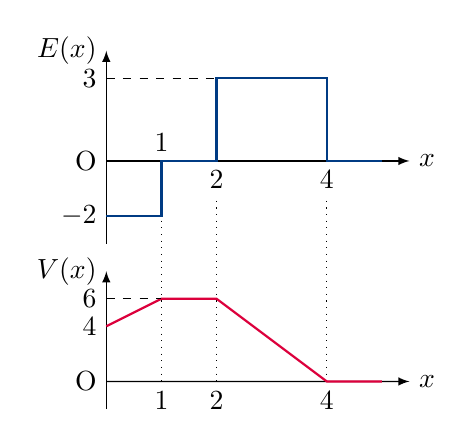
\begin{tikzpicture}[scale = 0.7]
          \coordinate (origin-e) at (0, 0);
          \coordinate (x-e) at ($(origin-e) + (5.5, 0)$);
          \coordinate (y1-e) at ($(origin-e) + (0, 2)$);
          \coordinate (y2-e) at ($(origin-e) + (0, -1.5)$);

          \coordinate (origin-v) at (0, -4);
          \coordinate (x-v) at ($(origin-v) + (5.5, 0)$);
          \coordinate (y1-v) at ($(origin-v) + (0, 2)$);
          \coordinate (y2-v) at ($(origin-v) + (0, -0.5)$);

          \draw[thin, dotted] ($(origin-e) + (1, 0)$) node[above]{$1$} -- ($(origin-v) + (1, 0)$) node[below]{$1$};
          \draw[thin, dotted] ($(origin-e) + (2, 0)$) node[below, fill=white]{$2$} -- ($(origin-v) + (2, 0)$) node[below]{$2$};
          \draw[thin, dotted] ($(origin-e) + (4, 0)$) node[below, fill=white]{$4$} -- ($(origin-v) + (4, 0)$) node[below]{$4$};

          \draw[thin, -latex] (origin-e) node[left]{O} -- (x-e) node[right]{$x$};
          \draw[thin, -latex] (y2-e) -- (y1-e) node[left]{$E(x)$};
          \draw[thin, -latex] (origin-v) node[left]{O} -- (x-v) node[right]{$x$};
          \draw[thin, -latex] (y2-v) -- (y1-v) node[left]{$V(x)$};

          \draw[thick, mri-blue] ($(origin-e) + (0, -1)$)
            -- ($(origin-e) + (1, -1)$)
            -- ($(origin-e) + (1, 0)$)
            -- ($(origin-e) + (2, 0)$)
            -- ($(origin-e) + (2, 1.5)$)
            -- ($(origin-e) + (4, 1.5)$)
            -- ($(origin-e) + (4, 0)$)
            -- ($(origin-e) + (5, 0)$);
          \draw[thin, dashed] ($(origin-e) + (0, 1.5)$) -- ($(origin-e) + (2, 1.5)$);
          \node[left] () at ($(origin-e) + (0, -1)$) {$-2$};
          \node[left] () at ($(origin-e) + (0, 1.5)$) {$3$};

          \draw[thick, mri-red1] ($(origin-v) + (0, 1)$)
            -- ($(origin-v) + (1, 1.5)$)
            -- ($(origin-v) + (2, 1.5)$)
            -- ($(origin-v) + (4, 0)$)
            -- ($(origin-v) + (5, 0)$);
          \draw[thin, dashed] ($(origin-v) + (0, 1.5)$) -- ($(origin-v) + (1, 1.5)$);
          \node[left] () at ($(origin-v) + (0, 1)$) {$4$};
          \node[left] () at ($(origin-v) + (0, 1.5)$) {$6$};
        \end{tikzpicture}

        \caption{電界と電位の関係}
      \end{figure}

    \end{column}

  \end{columns}

\end{frame}

\begin{frame}[t]
  \frametitle{基礎}
  \framesubtitle{抵抗率と温度}

  \textcolor{mri-blue}{
  \textbf{導線の抵抗値は物質ごとに温度で決定する抵抗率$\rho(T)$と導線の長さと断面積$L, S$で決定する。
  また、抵抗率と温度の関係については近似式が存在する。これらから、抵抗値と温度の関係を計算することができる。
  \vspace{1zh}
  }
  }

  導線の抵抗値$R(T)$は抵抗率$\rho(T)$と導線の長さと断面積$L, S$から次のように計算される。
  \begin{equation}
    R(T) = \rho(T) \cdot \frac{L}{S}
  \end{equation}
  また、室温付近では抵抗率と導線の温度関係は温度計数を$\alpha$とすると以下で近似される。
  \begin{equation}
    \rho(T) = \rho(T_{0}) \{ 1 + \alpha (T-T_{0}) \}
  \end{equation}
  同じ導線で議論している場合は、抵抗率をそのまま抵抗値に変換できる。
  \begin{equation}
    R(T) = R(T_{0}) \{ 1 + \alpha (T-T_{0}) \}
  \end{equation}
  温度差について式を解くと次のようになる。
  \begin{equation}
    T-T_{0} = \frac{1}{\alpha} \cdot \left( \frac{R(T)}{R(T_{0})} - 1 \right)
  \end{equation}

\end{frame}

\begin{frame}[t]
  \frametitle{基礎}
  \framesubtitle{電荷の運動に関わる力}

  \textcolor{mri-blue}{
  \textbf{電荷に加わる力は、電界によるものと磁界によるものの2つが存在する。電界による静電気力と磁界によるローレンツ力である。
  \vspace{1zh}
  }
  }

  \begin{columns}[t]
    \centering

    \begin{column}{0.55\textwidth}
      \textbf{電界による力}
      \vspace{1ex}

      正電荷は電界と同じ方向に力を受け、その大きさは電荷の大きさと電界の強さの積となる。
      \vspace{1zh}

      \textbf{磁界による力}
      \vspace{1ex}

      磁界により電荷に加わる力は、電荷が移動しているときに発生する。
      力の向きは電荷の移動方向と磁界の向きのそれぞれに垂直な方向である。
      多くの場合、磁界と電荷の移動方向が垂直な状況が出題されるため、力の大きさは
      電荷の大きさ、速度、磁界の強さの積である。
      \vspace{1zh}

      \textbf{ローレンツ力の向き(外積の方向)について}
      \vspace{1ex}

      外積の方向は右ねじの法則により求めることができる。
      外積の前のベクトルから後ろのベクトルへの回転方向に対して、      右ねじの法則を適応すると、外積ベクトルの方向が分かる。

    \end{column}

    \begin{column}{0.4\textwidth}
      \begin{figure}[t]
        \centering
        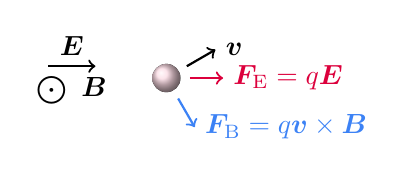
\begin{tikzpicture}[scale = 0.6]
          \coordinate (charge) at (0, 0);
          \coordinate (e-field) at (-2, 0.25);
          \coordinate (m-field) at (-2, -0.25);


          \fill[ball color=mri-red3] (charge) circle[radius=3mm];
          \draw[thick, ->] ($(e-field) - (0.5, 0)$) -- node[above]{$\bm{E}$} ($(e-field) + (0.5, 0)$);
          \node[] at (m-field) {$\bigodot\ \bm{B}$};
          \draw[thick, ->] (30:0.5) -- (30:1.2) node[right]{$\bm{v}$};

          \draw[thick, mri-red1, ->] (0.5, 0) -- (1.2, 0) node[right]{$\bm{F}_{\mathrm{E}} = q\bm{E}$};
          \draw[thick, mri-blue1, ->] (-60:0.5) -- (-60:1.2) node[right]{$\bm{F}_{\mathrm{B}} = q\bm{v}\times\bm{B}$};

        \end{tikzpicture}

        \caption{電界と磁界によって電荷に加わる力}
      \end{figure}

      \begin{figure}[t]
        \centering
        \includegraphics[width=0.38\textwidth]{./img/gaiseki.png}
        \caption{外積の向き
          (出所:高校数学.net 「空間ベクトルと外積」 \url{https://xn--48s96ub7b0z5f.net/kuukan-bekutoru-gaiseki/})
        }
      \end{figure}



    \end{column}

  \end{columns}

\end{frame}

\begin{frame}[t]
  \frametitle{基礎}
  \framesubtitle{円形コイルによる磁界}

  \textcolor{mri-blue}{
  \textbf{定常電流により発生する磁界に関して、ビオ・サバールの法則の理解が求められる。
  \vspace{1zh}
  }
  }

  \begin{columns}[t]
    \begin{column}{0.55\textwidth}
      \textbf{ビオ・サバールの法則}
      \vspace{1ex}

      微小な長さの電流要素$I\mathrm{d}\bm{l}$によって、
      $\bm{r}$離れた地点に発生する磁界$\mathrm{d}\bm{H}$は以下で計算される。
      \begin{equation}
        \mathrm{d}\bm{H} = \frac{I\mathrm{d}\bm{l} \times \bm{r}}{4\pi \lvert \bm{r} \rvert^{3}}
      \end{equation}

      \vspace{1zh}

      \textbf{円形電流による磁界}
      \vspace{1ex}

      図形の対称性から$z$成分のみに注目\footnote{積分計算で$x, y$成分が打ち消されるため。}し、ビオ・サバールの法則を適応する。
      \begin{equation}
          \mathrm{d} H_{\mathrm{z}}
          = \frac{I \cdot \lvert \bm{r} \rvert \cdot \mathrm{d}l}{4\pi \lvert \bm{r} \rvert^{3}} \cdot \sin\theta
          = \frac{I \cdot  \mathrm{d}l}{4\pi (\sqrt{a^{2} + z^{2}})^{2}} \cdot \frac{a}{\sqrt{a^{2} + z^{2}}} 
      \end{equation}
      \begin{equation}
        H_{z} = \frac{ Ia }{4\pi (a^{2} + z^{2})^{3/2}}  \int_{0}^{2\pi a} \mathrm{d}l = \frac{Ia^{2}}{2(a^{2} + z^{2})^{3/2}} 
      \end{equation}


    \end{column}

    \begin{column}{0.4\textwidth}

      \begin{figure}
      \begin{center}
        \begin{tikzpicture}[scale = 1.2]
          \coordinate (origin) at (0, 0);
          \coordinate (z) at (0, 1.5);

          \draw[thin] ($(origin) + (0, -1)$) -- (origin);
          \fill (origin) node[below left]{$\mathrm{O}$} circle[radius=2pt];
          \draw[line width=3pt, white] (268:0.5) arc[radius=0.5, start angle=268, end angle=272];

          \draw[thin, ->, name path=ellipse] ($(origin) + (0:1.5)$) node[right]{$I$}
            arc[x radius=1.5, y radius=0.5, start angle=0, delta angle=355];
          \draw[line width=3pt, white] (0, 0.45)--(0, 0.55);

          \draw[thin, ->] (origin) -- ($(origin) + (0, 2)$) node[above]{$z$};

          \draw[thin, latex-latex] (origin) -- node[below]{$a$} (180:1.5);

          \path[name path=line1] (z) -- (-60.5:2);
          \path[name path=line2] (z) -- (-59.5:2);
          \path[name intersections={of=ellipse and line1, by={q1, p1}}];
          \path[name intersections={of=ellipse and line2, by={q2, p2}}];
          \draw[thick, ->, mri-blue] ($(p1)!-10!(p2)$) -- node[below]{$\mathrm{d}\bm{l}$} ($(p1)!10!(p2)$);

          \draw[line width=3pt, white] ($(z)!0.45!(p2)$) -- ($(z)!0.55!(p2)$);
          \draw[thick, ->, mri-green1] (z) -- node[above right]{$\bm{r}$} (p2);

          \draw[thick, ->, mri-red1] (z) -- ($(z) + (25:0.5)$) node[above right]{$\mathrm{d}\bm{H}$};

          \fill[] (z) circle[radius = 2pt] node[left]{点P: $(0, 0, z)$};

          \draw[thin] ($(z)+(270:0.5)$) to[out=-60, in=240] node[below=5pt, right=-4.5pt]{$\theta$} ($(z)+(287:0.5)$);

        \end{tikzpicture}

      \end{center}
      \caption{円形電流による磁界}
      \end{figure}

    \end{column}

  \end{columns}

\end{frame}

\end{document}
